
\documentclass{beamer}


\mode<presentation>
{
  \usetheme{CambridgeUS}
	\usecolortheme{beaver}
  % or ...

  \setbeamercovered{transparent}
  % or whatever (possibly just delete it)
}


\usepackage{xeCJK}
\usepackage[english]{babel}
\usepackage[utf8]{inputenc}
\usepackage{times}
\usepackage[T1]{fontenc}
\usepackage{hyperref}
\usepackage{pifont}
\usepackage{bibentry}
\usepackage{verbatim}
\usepackage{color}
\newcommand{\cmark}{\ding{51}}%
\newcommand{\xmark}{\ding{55}}%
\setCJKmainfont{WenQuanYi Micro Hei}
\renewcommand{\raggedright}{\leftskip=0pt \rightskip=0pt plus 0cm}
\raggedright

\let\oldfootnotesize\footnotesize
\renewcommand*{\footnotesize}{\oldfootnotesize\tiny}


\title[开源软件基础] 
{开源软件基础}
\subtitle{基于MongoDB的半结构化存储}

\author[Zhilei Ren] 
{Zhilei Ren}

\institute[OSCAR Team] % (optional, but mostly needed)
{
\\
\includegraphics[width=0.2\textwidth]{../../utils/logo.jpg}\\
OSCAR Team, School of Software, 
Dalian University of Technology
}


\subject{Scientific Writing}



\pgfdeclareimage[height=0.5cm]{university-logo}{../../utils/logo.jpg}
\logo{\pgfuseimage{university-logo}}



% Delete this, if you do not want the table of contents to pop up at
% the beginning of each subsection:
\AtBeginSubsection[]
{
  \begin{frame}<beamer>{Outline}
    \tableofcontents[currentsection,currentsubsection]
  \end{frame}
}


% If you wish to uncover everything in a step-wise fashion, uncomment
% the following command: 

%\beamerdefaultoverlayspecification{<+->}

\setbeamertemplate{section in toc}[circle]
\setbeamertemplate{items}[circle]
\setbeamertemplate{caption}[numbered]
\setbeamertemplate{bibliography item}{\insertbiblabel}
\setbeamertemplate{bibliography entry title}{}
\setbeamertemplate{bibliography entry journal}{}

\begin{document}

\begin{frame}
  \titlepage
\end{frame}

%\begin{frame}{Outline}
%  \tableofcontents[currentsection,currentsubsection, 
%    hideothersubsections, 
%    sectionstyle=show,
%]
%\end{frame}

\AtBeginSection[]
{
 \begin{frame}<beamer>
 \frametitle{Outline}
 \tableofcontents[currentsection]
 \end{frame}
}
\section{MongoDB}
\begin{frame}[t]{NoSQL简介}
\end{frame}
\begin{frame}[t]{MongoDB简介}
\end{frame}
\begin{frame}[t]{MongoDB基本使用}
	\centering
	
\includegraphics[width=.4\textwidth]{mongodb.png}
	\begin{block}{Intro}
		\small
		MongoDB是一种文档导向的数据库管理系统，由C++撰写而成，以此来解决应用程序开发社区中的大量现实问题。2007年10月，MongoDB由10gen团队所发展。2009年2月首度推出\footnote{\url{https://zh.wikipedia.org/zh-cn/MongoDB}}。
	\end{block}

	\Huge
	{\color{red}Mongo} for \pause hu{\color{red}mongo}us
\end{frame}
\begin{frame}[t]{MongoDB REPL}
	\begin{block}{REPL}
		\small
		\begin{itemize}
			\item Read Evaluate Print Loop
			\item 在现代语言中非常流行
			\item MongoDB的REPL基于JavaScript
		\end{itemize}
	\end{block}
	\centering
	\begin{figure}
		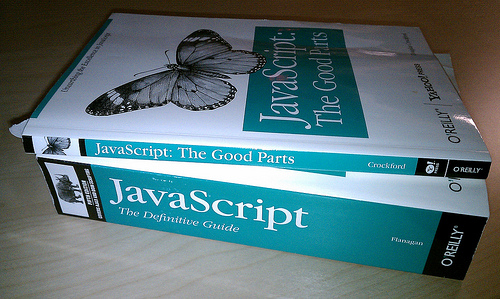
\includegraphics[width=.4\textwidth]{definitive-vs-good.jpg}
		\caption{The definitive guide vs. the good part}
	\end{figure}
\end{frame}
\begin{frame}[t]{MongoDB数据结构}
\end{frame}
\section{基于pymongo的数据库连接}
\begin{frame}[t]{pymongo简介}
\end{frame}
\begin{frame}[t]{pymongo安装}
\end{frame}

\begin{frame}[fragile]{pymongo API使用}
	\begin{block}{Python snippet}
\begin{verbatim}
import pymongo
from pymongo import MongoClient
client = MongoClient()

# Get the sampleDB database
db = client.sampleDB 
# equivalently, use db = client['sampleDB']
coll = db.sampleCollection
# equivalently, use coll = db['sampleCollection']
\end{verbatim}
	\end{block}
\end{frame}

\begin{frame}[t]{pymongo API使用}
\end{frame}

\end{document}
